\chapter{Introduction}
\label{chap:Introduction}

\section{Background \& Motivation}
\lettrine[findent=2pt]{{\fbox{\textbf{T}}}}{ }he fast-paced development of Intelligent Transportation Systems (\textit{ITS}) forms one cornerstone in the context of modern Smart Cities, allowing to upgrade the existing standards in managing traffic, planning urban areas, ensuring public safety, and taking care of environmental concerns.

It wasn't until the rise of Artificial Intelligence, along with Deep Learning techniques \cite{CityFlow, AggregatingGlobalLocal, MultiLevelProgressiveLearning}, that Traffic Management ceased from being based on fixed-time traffic signals, human-operated operations, and static road infrastructure designs. Let's, for example, think about a traffic officer stationed at the middle of a junction, who used hand and body movements to control vehicle flow or an early traffic surveillance system that required a human operator to actually detect congestions or accidents within CCTV cameras. Data collection for traffic patterns included labor-intensive vehicle counts and road designs and optimized signal timings were manually annotated, revised and studied. These systems, however, although being reactive in nature, were also commonly prone to errors, with a limited ability to adapt to the dynamic and unpredictable nature of urban traffic. These limitations, further aggravated by human judgments based on static systems, made it very inefficient and raised a strong need for more automated and independent solutions. With the recent unstoppable progress in the technological field, AI-driven solutions have been successfully integrated into this domain \cite{SelfSupervisedGeometricFeatures, MsKAT}, making traffic management real-time, scalable and predictive, thus addressing and overcoming the shortcomings of conventional approaches. These new systems apply modern techniques of Computer Vision and Artificial Intelligence to automate the analytics of video feeds from extensive city-wide camera networks, thereby extracting crucial insights that support immediate decisions and long-term urban enhancements.

\section{Vehicle Re-Identification}
Vehicle Re-Identification (Re-ID) is a very specific and important subdomain of the object and person Re-ID domain, which lies on the association of the same vehicle images, captured from different camera views, under various conditions. In other words, the task involves assigning consistent IDs to vehicles across a network of surveillance or traffic cameras (CCTV), often in the presence of diverse environmental challenges and barriers. The valuable significance of Vehicle Re-ID is that it finds a wide range of practical applications, especially in ITS, urban traffic monitoring, public safety and security \cite{DeepHiddenMultiViewInference}. For example, it could be essential in tracking stolen vehicles, managing traffic flow across city networks  and monitoring transportation infrastructure for optimization and security purposes.

The difficulty of Vehicle Re-ID is that the real-world conditions do impose unique challenges for this domain \cite{EfficientBaseline, BagOfTricks, Glamor}. Vehicles can have \textbf{large intra-class variations}, for example, where the same exact car may look very different under different illuminations, weather conditions, camera viewpoints and occlusions as in \ref{fig:IntraInterClass}. On the other hand, \textbf{small inter-class differences} capture almost-identical vehicles of the same make, model and color, which make the task even more difficult thanks to the subtle and elusive visual differences. These factors necessitate the development of advanced techniques capable of extracting and leveraging fine-grained details to enable robust identification.

% Intra/Inter-Class Image
\begin{figure}[ht]
    \centering
    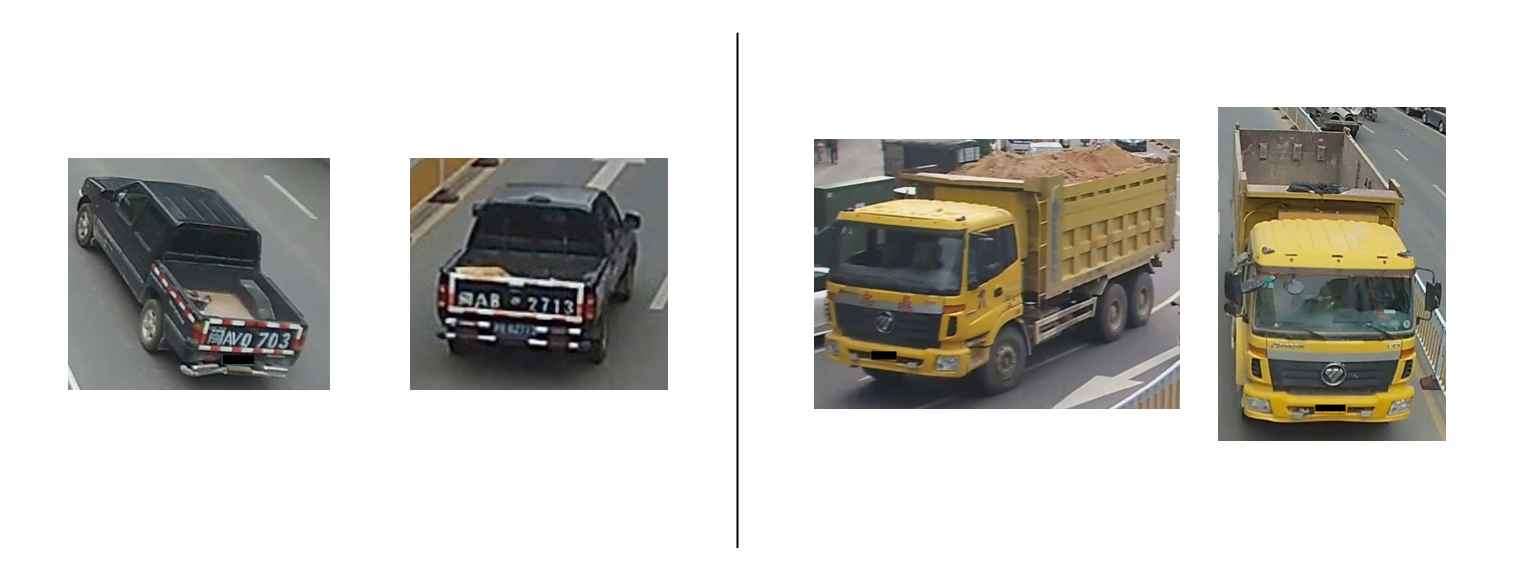
\includegraphics[width=1.0\textwidth]{images/IntraInterClass.jpg}
    \caption[Intra-Class \& Inter-Class Variations]{An example of inter-class variations (left) and intra-class differences (right). Note the missing top dust on the yellow truck.}
    \label{fig:IntraInterClass}
\end{figure}

Furthermore, the importance of Vehicle Re-ID extends beyond technological curiosity, as it directly addresses several pressing real-world needs. In urban environments with increasing transportation networks, the ability to track vehicles in a seamless manner across multiple non-overlapping camera feeds is invaluable. Traditional surveillance systems rely on either human operators or other manual ways, which mostly fail when it comes to scaling in volume and complexity of today's traffic systems. Vehicle Re-ID systems not only alleviate this burden but provide real-time, automated and scalable solutions that will drive smarter urban mobility, effective law enforcement and higher traffic efficiency.

With the advent of Deep Learning, Vehicle Re-ID has undergone a paradigm shift, exploiting the power of Convolutional Neural Networks (CNNs) in order to address these challenges \cite{MultiAttributeSpatialTemporal, LearningCoarseStructuredFeature, VRIC2}. CNNs, with architectures like ResNet or VGG, have been proved to be particularly effective in learning hierarchical and discriminative features from general visual data. Unlike traditional methods such as Template Matching, CNNs automatically learn features from diverse visual conditions that make them robust to changes in viewpoint, lighting, and occlusions. These have brought remarkable improvements in performance, allowing for reliable identification under challenging scenarios, which are really common in this domain.

Despite these breakthroughs, though, the task remains far from trivial. This is due to the fact that access to large-scale and high-quality datasets is required to train effective Vehicle Re-ID Neural Networks on generalizing the given task throughout different conditions. Besides that, feature extraction methods should ideally be able to capture fine-grained details, so that their system can identify minute-level differences while still being intra-class variation-robust. Most of recent works, which will be later discussed in Chapter 2, rely on sophisticated architectures that combine \textbf{global} and \textbf{local} feature representation \cite{VehicleReID_1, VehicleReID_2, VehicleReID_3}, ensuring that critical attributes like unique shapes, textures, or decorations are well-represented and used effectively for identification.

Ongoing research in Vehicle Re-ID is aimed at closing the gap between existing capability and real-world demand. This involves not only improving accuracy and robustness, but also ensuring that the systems are scalable, efficient and deployable in resource-constrained scenarios, such as deplying the system on Edge devices (TPUs for example). By leveraging innovations in Deep Learning, such as advanced CNN architectures and detailed attention mechanisms, researchers continue to push the boundaries of what is possible in Vehicle Re-ID, bringing us closer to smarter and safer transportation systems that are integral to the vision of modern smart cities.

\section{Multi-Target Single-Camera Tracking}
Multi-Target Single-Camera Tracking (\textit{MTSC}) \cite{RealTimeMultiObjectTracking, FairMOT} represents a pivotal step for most re-identification systems. It's an essential baseline for robust Object Tracking when dealing with an input coming one camera only. This tracking-by-detection paradigm effectively tracks multiple objects in a single video sequence with the use of object detections. Thus, the major task in MTSC is maximizing True Positives (TP) while minimizing False Positives (FP), False Negatives (FN), and ID switches.

The essence of MTSC can be appreciated when Multi-Target Multi-Camera Tracking (\textit{MTMC}) kicks in, which will be explained in the next section, because the true role in the pipeline is to try and keep object identities right and consistent throughout the video. Talking about consistency, an ID switch in which a previously tracked object gets a new identity can, in fact, have catastrophic consequences for the final results, such as a complete loss of a vehicle's trajectory. This is particularly problematic for scenarios where occlusions by other vehicles, trees or building structures are very common. This disruption of the vehicle's trajectory is able to make the subsequent re-identification process quite challenging, if not almost impossible. An example of ID switch is shown in \ref{fig:Unification}.

To tackle down this issue and all the problems related to it, the tracking algorithm should be strong and able to adapt to complex scenarios that essentially occur in reality. It should handle occlusions, sudden changes in motion, and overlaps of objects without compromising the accuracy of results. Advanced approaches have been used, integrating motion models with appearance-based feature matching in order to alleviate such issues. Moreover, this step requires a very precise detection methods because inaccuracies in bounding box localization or classification may result in the whole tracking pipeline having errors. With a good MTSC system, vehicles are guaranteed to be consistently tracked within the same camera feed, laying a strong foundation for the Multi-Target Multi-Camera Tracking task.

\section{Multi-Target Multi-Camera Tracking}
Building on the work done by the MTSC algorithm, the Multi-Target Multi-Camera Tracking (\textit{MTMC}) \cite{He2019MultiCameraVT, MTMCTrajectoryBased1, pahel2019VehicleRA, ELECTRICITY} concept extends this tracking phase to multiple, usually non-overlapping, camera feeds. This is of paramount importance in ITS for achieving a comprehensive understanding of vehicle movement across a city or any large-scale environment. MTMC, then, enables various applications, including real-time traffic management, city-wide security monitoring, and the efficient oversight of the transportation infrastructures.

The complex challenge of linking vehicle trajectories across cameras lies at the heart of MTMC. This involves overcoming a lot of technical hurdles, such as changing viewpoints of cameras, inconsistent lighting conditions, occlusions, and environmental factors like weather or even camera malfunctions. Vehicle ReID plays a central role in MTMC, as it ensures that the same vehicle is correctly identified and tracked across different camera feeds. The success of MTMC heavily relies on integrating robust trajectory linking methods, which could successfully associate trajectories based on the principles of spatial proximity, temporal coherence and directional consistency.

Within MTMC, Multi-Camera Vehicle Re-Identification (ReID) has become a domain of precise and careful consideration. This field aims to accurately seek the correct identification and tracking of the same vehicle in several cameras while mitigating some huge technical hurdles like variable lighting conditions, angles of cameras, occlusions and other environmental factors, like weather conditions.

Trajectory clustering \cite{MTMCTrajectoryBased1} is of fundamental importance in MTMC, as vehicle trajectories in different cameras are combined together based on spatial, temporal and directional constraints. This procedure ensures that the same vehicle obtains consistent identity across several feeds and in order to pursue an effective success, precise synchronization and calibration of cameras is also needed. Precise timestamp alignment and geometric calibration among cameras enable the system to map trajectories across distinct fields of view (FOV) seamlessly. In addition, the robustness of the Object Detector and Feature Extractor in the earlier MTSC stage significantly influences the overall performance of MTMC. Discriminative features and high-confidence bounding boxes ensure that the re-identification process is reliable and scalable, even when occlusions and environmental noise are present.

In MTMC systems, robustness is not a luxury but a must-have. The entrance and exit of vehicles in the field of view of different cameras take place under different conditions, thus, a system must be able to compensate for partial or even missing data. With this general idea of building such a system, vehicle tracking and re-identification will benefit from high accuracy, even under such complicated conditions, further enhancing the system's applicability in real-world ITS scenarios. MTMC, then, tries to bridge the gap between individual camera feeds and provides a more complete view of vehicle movements, offering a transformative tool for modern urban planning and security applications.

\section{Research Objectives}
This thesis addresses two of the key challenges in the Vehicle ReID pipeline:
\begin{itemize}
    \item \textbf{Feature Extraction:} The ability to extract discriminative features from vehicles, via Deep Learning techniques, that are invariant to changes in viewpoint, illumination, and occlusions.
    \item \textbf{MultiTrack Re-Identification:} The ability to re-identify vehicles across multiple cameras through linking of their trajectories based on spatial, temporal, and directional constraints.
    \item \textbf{Target Vehicle Search:} The ability to filter vehicles based on color characteristics and patterns of movement, to focus on specific vehicles of interest.
\end{itemize}

The process starts with a frame-by-frame processing, per camera, through YOLO-based Detection and Tracking. YOLO processes these frames with a resolution of (640, 640) and it's able to generate Bounding Boxes along with an initial ID assignment. This approach is crucial, since a robust detection and tracking system is the first step in the pipeline. Especially, the Detection Model needs to properly identify the vehicles in the scene, taking into account the different problems that might arise throughout the whole camera network.
Furthermore, the Tracking Model which, for this project, is either BOTSort or ByteTrack, must have the capacity to appropriately follow the vehicles in the scene, even when they are occluded. This is a big issue when it comes to tracking, since most of the time vehicles are occluded by other vehicles, trees, buildings, etc. and the Tracklet might be lost forever, subsequently assigning a new ID to the same vehicle (this is known as ID switching).

In this case, we do define a Tracklet as the basic unit of tracking. It's a sequence of detections, for a unique car, that are linked together by the tracking algorithm, representing the trajectory of the vehicle in the scene.

Frames are then filtered to retain only high-confidence ones to ensure data quality and thus reducing noise in any further analysis.
Distinctive vehicle features are extracted by employing a deep ResNet50-based feature extraction model trained on large-scale datasets of vehicle images (VeRi-776, VehicleID, AICity) with advanced training techniques to adapt it to the considered domain. These techniques mainly focus on loss functions like Triplet Loss, Supervised Constrastive Loss and RPTM (\textit{Relation Preserving Triplet Mining}), which is crucial for the model for learning the features that are most discriminative.

All the processed frames are then logged in detail with the following metadata:
\begin{itemize}
    \item Frame number
    \item Vehicle ID
    \item Compressed Image (for later visualization)
    \item Bounding Box
    \item Confidence Score
    \item ResNet Features
    \item Shape (for later visualization)
    \item Timestamp
\end{itemize}

This data is systematically stored in a MongoDB database, hence forming a strong base for the vehicle re-identification task across multiple camera feeds, which will be later on based on feature similarity, temporal alignment, and directional consistency. The tracking results are further refined by an advanced unification algorithm which corrects misassignments in the initial Tracking phase using analysis of bounding box areas and timestamps. This simple and effective strategy significantly improves the overall tracking performance compared to standard detection and tracking methods. Finally, a unique feature vector for each vehicle is generated by averaging the stacked feature vectors and the system, then, computes the cosine similarity across vehicles in different camera feeds using ranked clustering with temporal and spatial constraints to ensure a correct reidentification.

On top of its core vehicle re-identification capabilities, the pipeline integrates advanced filtering mechanisms to only focus on specific vehicles of interest. The system allows the user to track vehicles selectively, according to their color characteristics and patterns of movement, filtering out all stationary vehicles and those with incomplete or unreliable detections. This is especially useful for applications of targeted tracking in which attention is concentrated on specific vehicles rather than an analysis of the flow of traffic in general, as for example in trying to locate the path of a stolen vehicle. The filtering step is multistage: first, it identifies and removes the stationary vehicles that stay virtually still beyond a given threshold, as these often represent parked cars or false detections; the second part filters out incomplete or partially visible bounding boxes for which feature extraction might be unreliable. Lastly, and perhaps most importantly, it can filter vehicles based on color using an EfficientNet-based color classifier or a ResNet+SVM approach for accurately recognizing the color of vehicles. Color-based filtering comes in handy, during the tracking of vehicles with particular colors, for police or security applications, as this helps to reduce the search space and computational overhead and at the same time it increases precision in targeted vehicle tracking.

The research work presented here contributes to continuous development within Intelligent Transportation Systems, but also considers practical and computational issues that arise in large-scale vehicle tracking, especially when it comes to a single target-vehicle tracking. Therefore, the main contribution of this work is to develop advanced Deep Learning methods with the establishment of a system capable of robust cross-camera vehicle recognition and target vehicle recognition, enabling a wide range of applications related to monitoring urban traffic and public safety for smarter, safer, and more efficient cities.

\section{Thesis Structure}
This introductory chapter has given an overview of the research context, the challenges in Vehicle Re-ID and the importance of Multi-Target Single-Camera and Multi-Target Multi-Camera Tracking in the context of Intelligent Transportation Systems. The technical aspects of the research will be taken up in the subsequent chapters. More formally, the study will be structured as follows:
\begin{itemize}
    \item \textbf{Chapter 2} will provide, for this scenario, a detailed review of the related works in the literature, as well as a presentation of state-of-the-art models in Object Detection and various robust Vehicle Re-ID algorithms.
    \item \textbf{Chapter 3} will outline the methodology, technical specifications and improvements of the proposed system, including the datasets used, the structural architecture design of the feature extraction model, object detection and tracking algorithms and, finally, the complete re-identification pipeline.
    \item \textbf{Chapter 4} will explain the experimental results and evaluation of the system in the feature extraction step and the re-identification step, including the filtering mechanisms and the color classification model.
    \item \textbf{Chapter 5} will conclude the thesis with a summary of the contributions, limitations, and future research directions in this field.
\end{itemize}
